\begin{figure}
    \centering
    \begin{minipage}{0.65\textwidth}
        \centering
        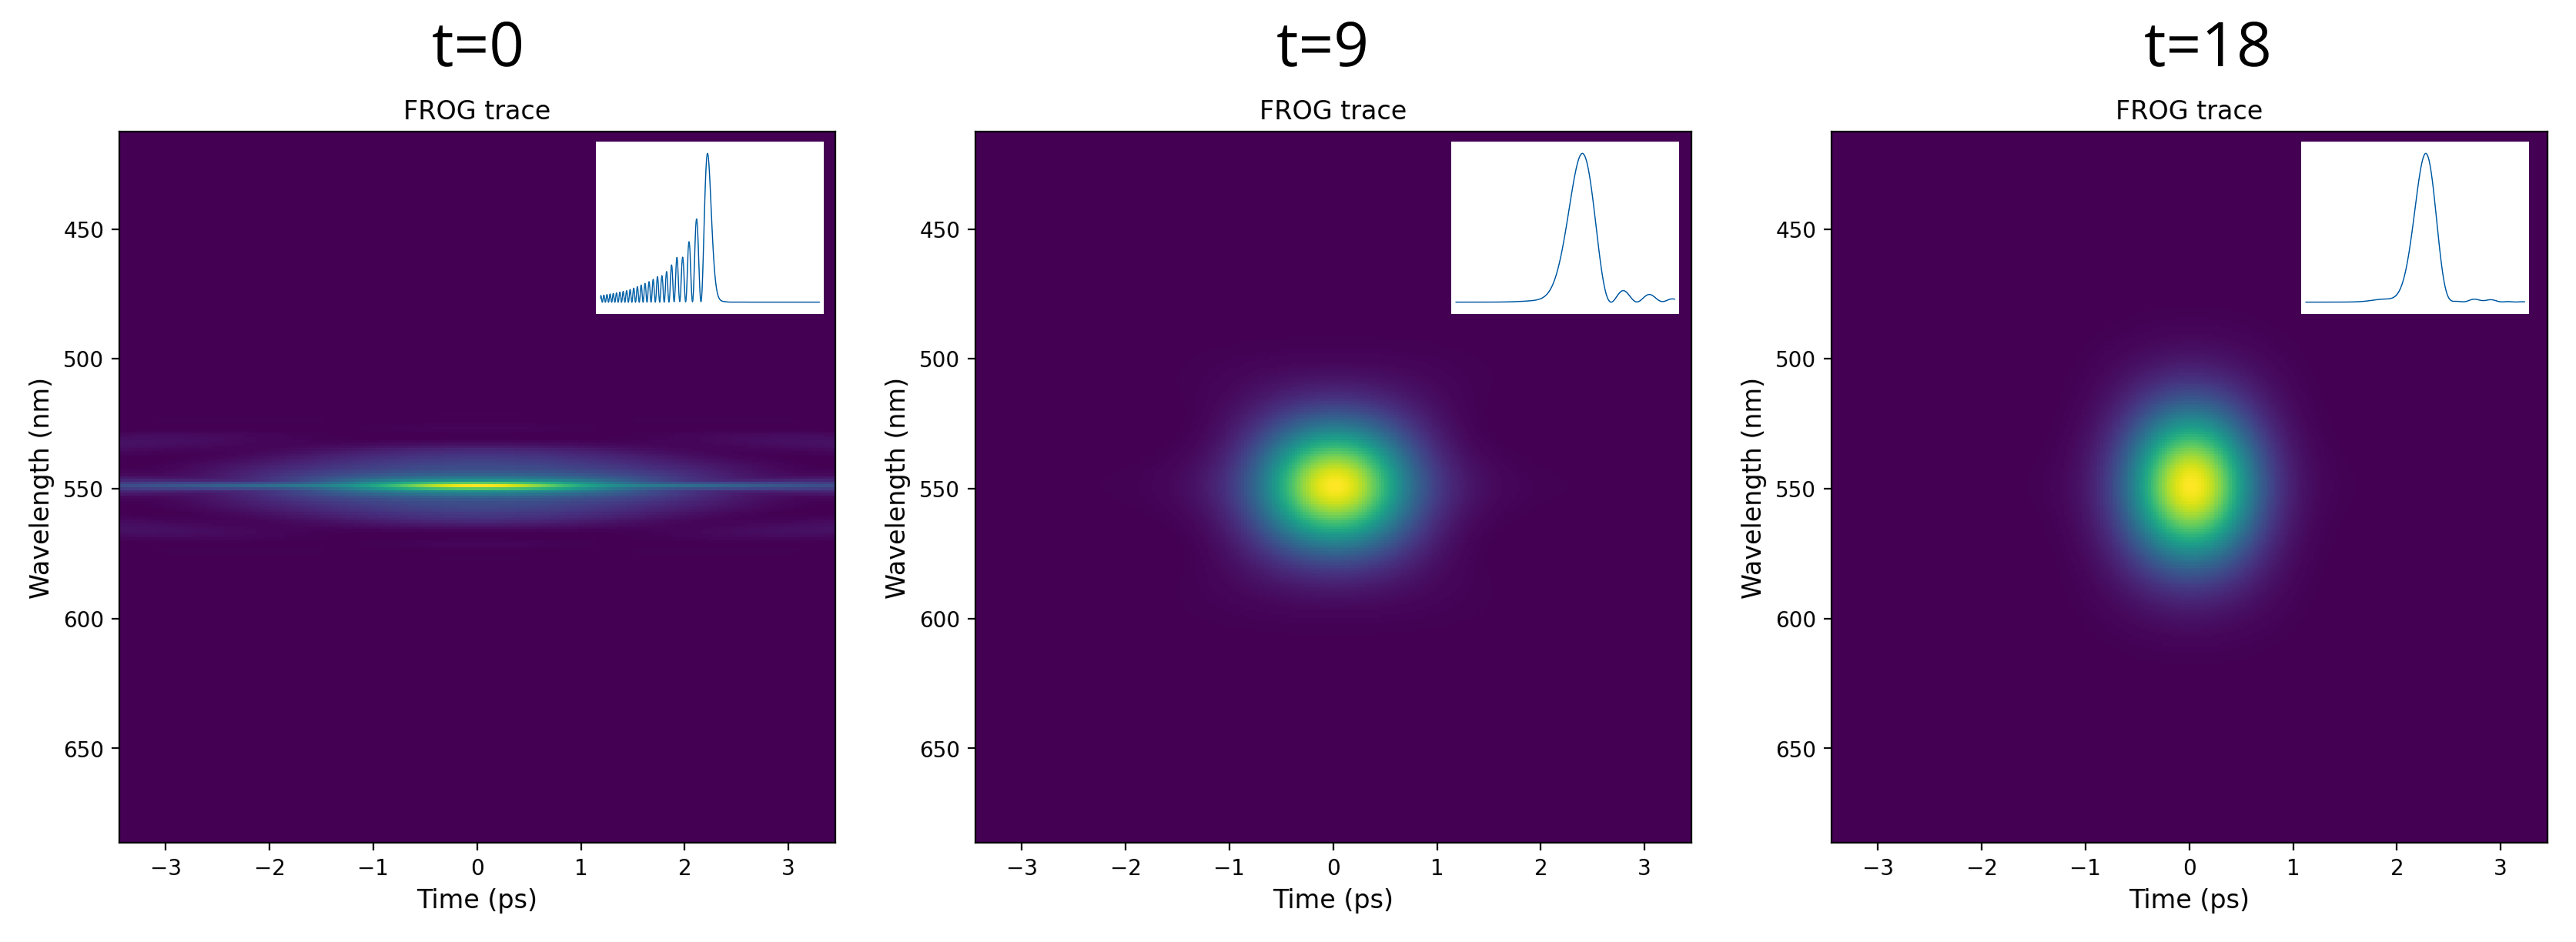
\includegraphics[width=\linewidth]{images/frogopt.png}
        \caption{SAC, learning to shape temporal pulses directly from FROG traces. The temporal profile associated with the FROG trace is superimposed on the top right of the trace for visualization purposes, and is never made available to the agent. In under 20 interactions, the agent produces near-TL temporal profiles.}
        \label{fig:frog_opt}
    \end{minipage}
    \hfill
    \begin{minipage}{0.30\textwidth}
        \centering
        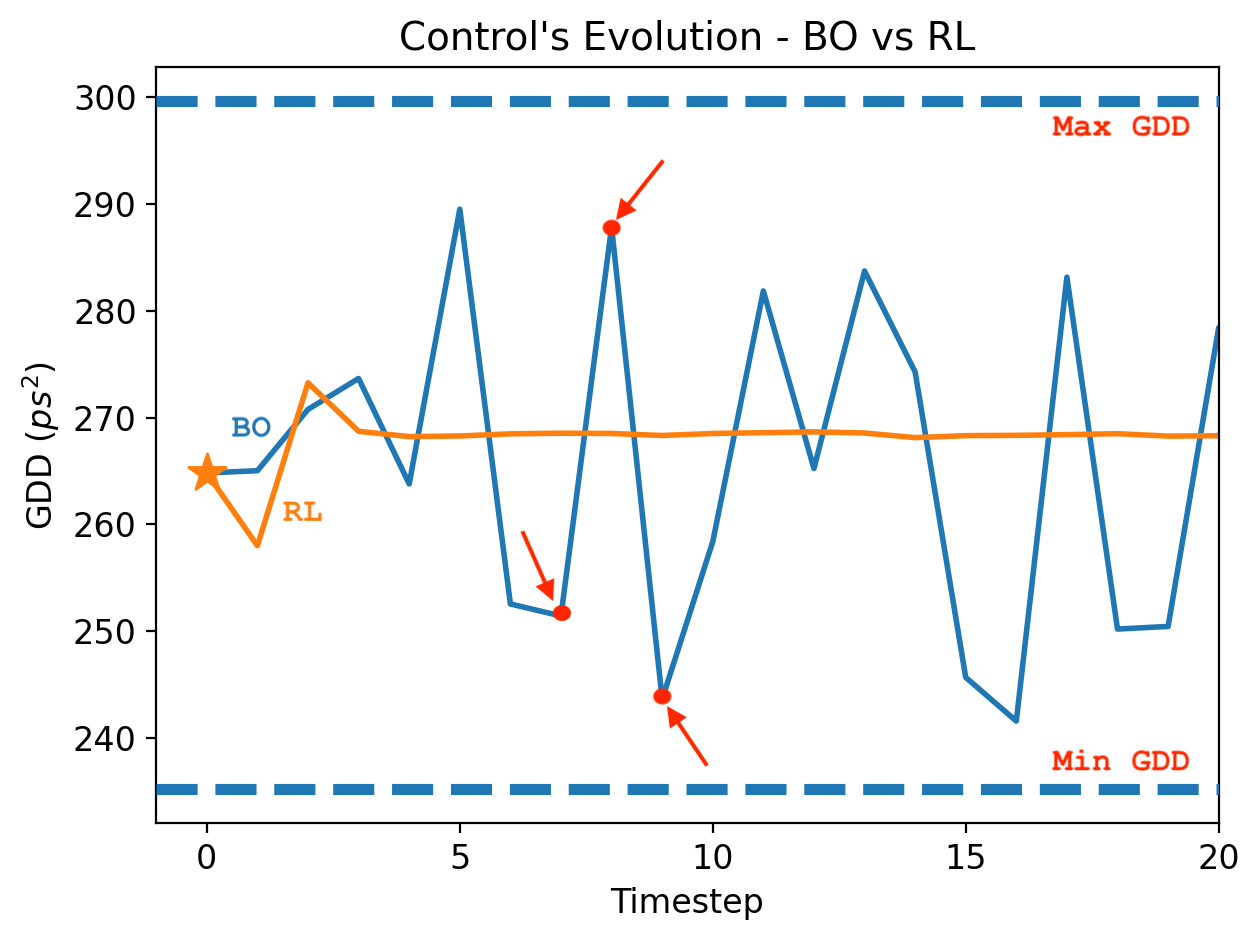
\includegraphics[width=\linewidth]{images/machinesafety.png}
        \caption{Controls applied (BO vs RL). As it samples from an iteratively-refined surrogate model of \( f(\psi)=I^*\), BO explores much more erratically than RL.}
        \label{fig:bayes_vs_rl}
    \end{minipage}
\end{figure}

\begin{figure}
    \centering
    \begin{minipage}{0.48\linewidth}
        \centering
        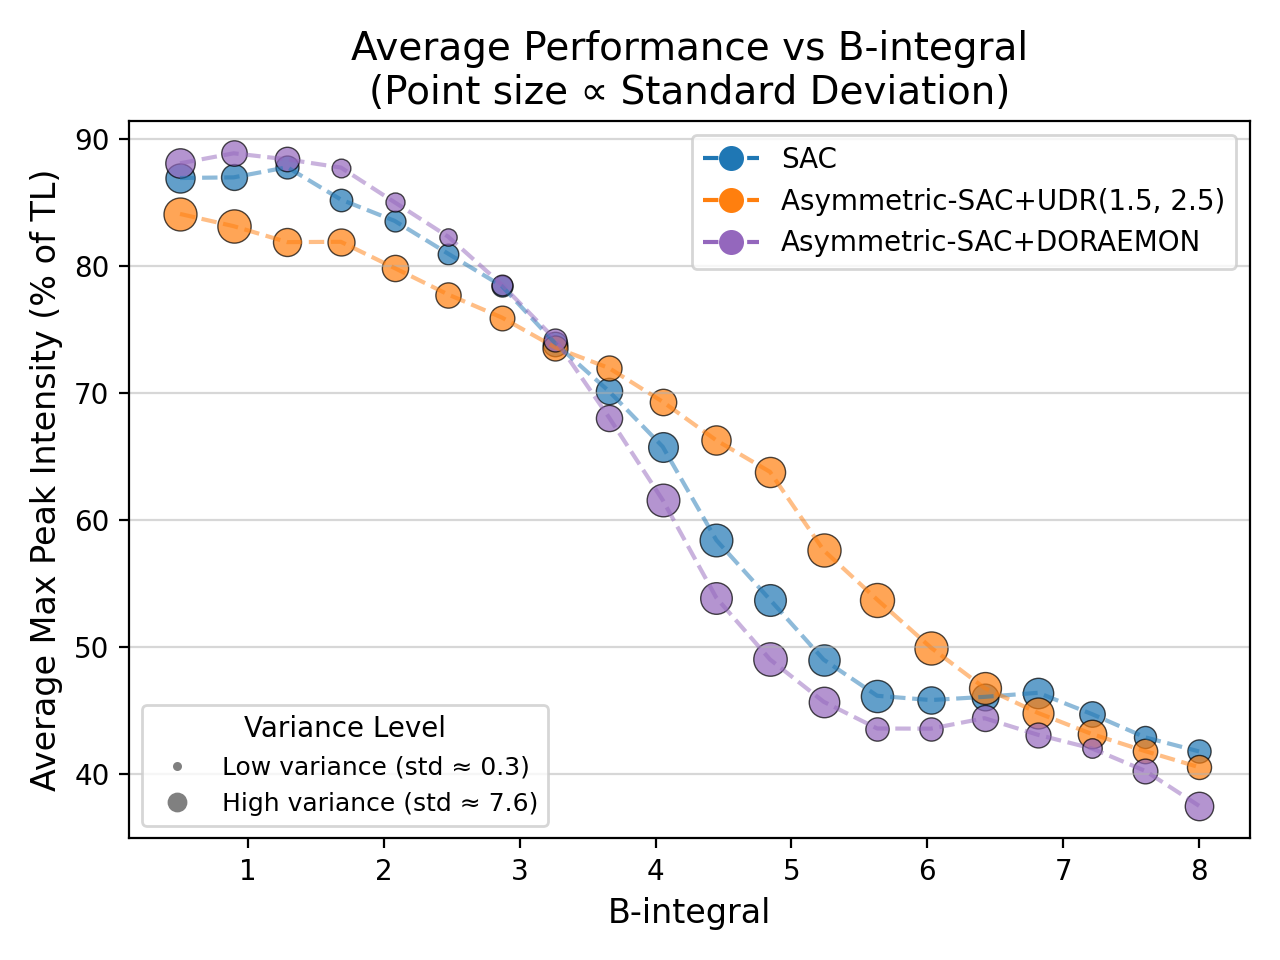
\includegraphics[width=\linewidth]{images/max_intensity_vs_b_integral.png}
        \caption{Comparison of different strategies, measured by the average max peak intensity over 5 test episodes as a function of B-integral. These results illustrate DORAEMON's comparable performance with hand-tuned bounds for UDR.}
        \label{fig:max_intensity_vs_b_integral}
    \end{minipage}
    \hfill
    \begin{minipage}{0.48\linewidth}
        \centering
        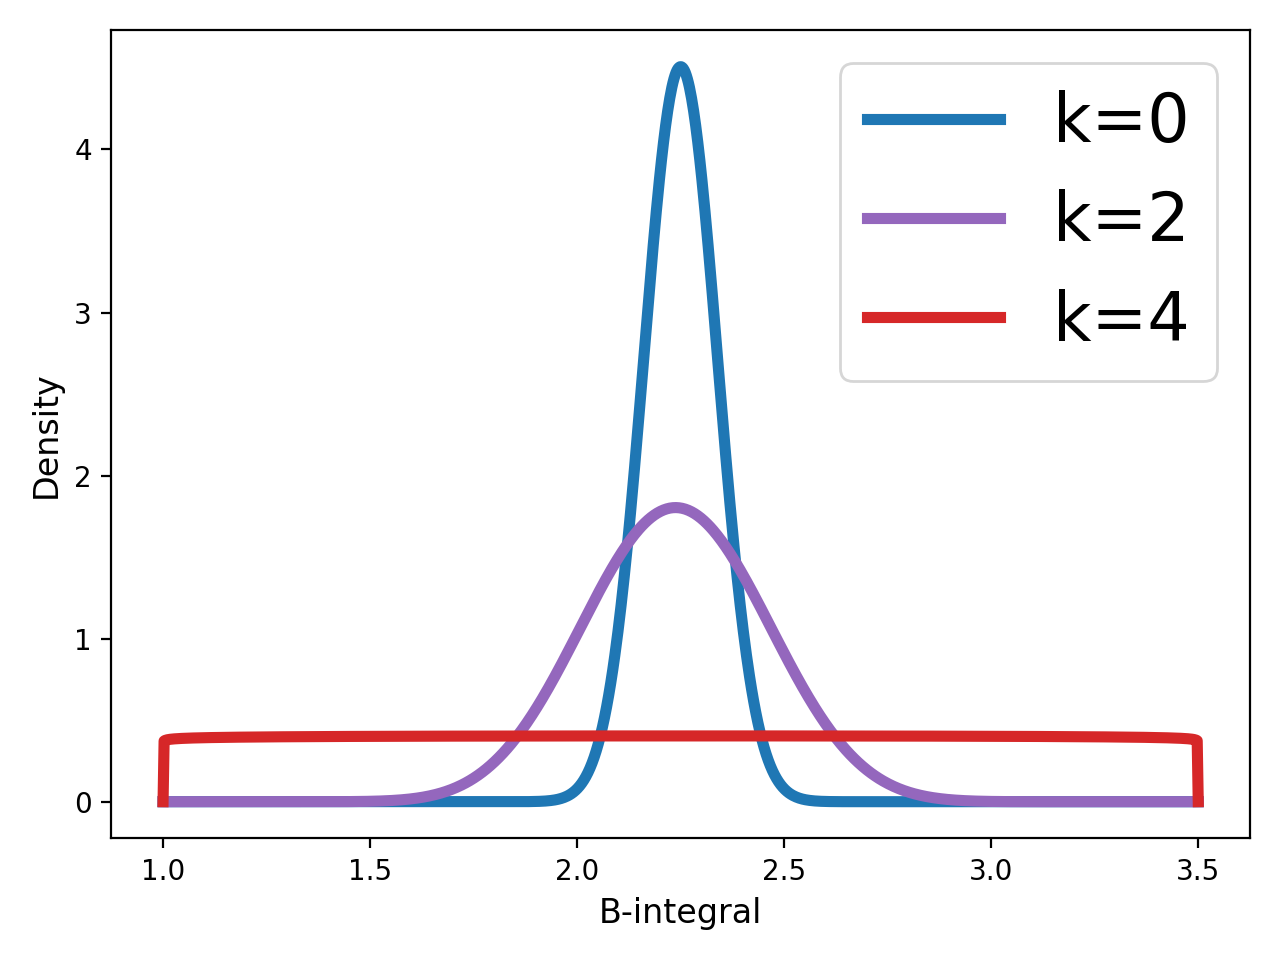
\includegraphics[width=\linewidth]{images/doraemon_distributions_3in1.png}
        \caption{Evolution of the distribution used when training an agent with DR via Entropy Maximization (DORAEMON). Later updates $20 \geq k \geq 4$ do not further impact the evolution of the distribution over $B$.
        %, as success rate plateaus at 90\%.
        }
        \label{fig:DORAEMON_distrs_over_training}
    \end{minipage}
\end{figure}

We validate our claims on the improved machine-safety of RL over popular baselines such as BO~\citep{shalloo2020automation} by comparing the evolution of the controls applied at test time for the both BO and \emph{mini-SAC}. As BO cannot be used to process images, we benchmark it against a simplified version of our algorithm that uses exclusively $\psi$ in the state vector, which we refer to as mini-SAC. Figure~\ref{fig:bayes_vs_rl} displays the evolution of the controls applied over the first 20 interactions between BO and the RL-based controller. Unlike BO's solutions, which are stationary and can only be transferred assuming high-fidelity simulations, RL policies can be transferred across domains and adapt at test time, leveraging a sequential decision-making framework.
%we can work on transferring control policies across domains.
Notably, this allows us to allocate dangerous erratic exploration to in-simulation training, severely limiting erratic exploration at test time---similarly to established work in robotics~\citep{kober2013reinforcement}. 
% As mini-SAC shares the same action space defined in~\ref{sec:mdp}, it is trained to never apply actions larger than 10\% of the total control range, resulting in more gentle control---significantly more suited for applications to real-world dynamical systems.

Since temporal profiles $\chi(\psi)$ are typically unavailable, we exclusively use 64x64 single-channel images as state representations for the agent, as discussed in~\ref{sec:mdp}. 
Table~\ref{tab:peak_intensities} shows the average max peak intensity over 10 test episodes, after training SAC for 200k timesteps in simulation on a fixed \( \xi \sim \delta(B_{\text{est}}) \), while Figure~\ref{fig:frog_opt} shows the FROG traces corresponding to the controls applied during a test episode at various timesteps. Effectively, the policy exhibits the capability of controlling $\psi$ to compress the pulse in time, achieving an average of 86.2\% of TL's peak intensity, with peaks close to 90\%(~\ref{tab:max_peak_intensities}). These findings also attest the effectiveness of using single-channel images as affordable proxy input to maximize peak intensity.

%After having tested the effectiveness of using single-channel images as direct inputs to maximize intensity,
Later, we benchmark the robustness of our policy to changes in the dynamics.
%Clearly, all configurations struggle on high levels of B (\( B \geq 3.5 \)).
%,while Asymmetric-SAC coupled with DR seems to do better on diverse values in the range \( [1, 3.5]\).
Particularly, we employ DR during training, and use Asymmetric-SAC together with a stack of the last $n=5$ states, yielding a history-based policy. This has shown to be effective in the context of DR to promote adaptive, meta-learning behavior~\citep{chen2021understanding, tiboni2023domain, akkaya2019solving}.
% Figure~\ref{fig:max_intensity_vs_b_integral} shows the average maximal peak intensity obtained by polices trained per Table~\ref{tab:peak_intensities}.
We evaluate the performance of our method by measuring the average max intensity versus equally-spaced changes in the value of B-integral (cf.~Figure~\ref{fig:max_intensity_vs_b_integral}). We then zoom in on these values, and report in Table~\ref{tab:peak_intensities} the average peak intensity for the test conditions within \( [1, 3.5] \) (i.e., in distribution contexts). When trained with DR, Asymmetric-SAC expectedly exhibits stronger robustness to changes in the parametrization of the test environment. However, performance varies significantly based on the distribution used while training, motivating the use for automated DR methods---Table~\ref{tab:peak_intensities} shows the impact of choosing narrower rather than wider bounds for UDR, as we find wider UDR to cause over-regularization, hindering performance at test time.
% Conversely, DORAEMON iteratively updates the distribution bounds in a curriculum fashion, resulting in better performance within a similar support.
We therefore compare the naive UDR approach with DORAEMON, by adapting the training distribution \( \{ \Xi_{k} \}_{k=1}^K\) across $K=20$ steps over 200k timesteps. Compared to UDR, DORAEMON displays better test-time performance around our estimate $B_{\text{est}} = 2$, and generally provides superior success rate (cf.~Table~\ref{tab:succ_rate}).
% It's worth noting that DORAEMON distributions still converge to uniform distributions along the process.
% We therefore attribute the stronger performance to the capabilities of the curriculum to avoid abrupt changes to the dynamics while training our policies with DR,
Figure~\ref{fig:DORAEMON_distrs_over_training} shows the evolution of the distributions \(\{\Beta(a_k, b_k) \}_{k=1}^{K} \) over the course of training.
%, when these are updated towards maximum entropy so long as a performance lower bound is maintained.
Interestingly, the distributions eventually converge to the maximum entropy \( \mathcal U(1, 3.5) \), indicating that sufficient training performance can be maintained even in the extreme case. To investigate the effectiveness of the curriculum for DORAEMON, we then evaluate it against naive UDR on a slighly narrower support \( \mathcal U(1, 3) \), and observe DORAEMON's superior in Table~\ref{tab:peak_intensities}).

% \begin{table}[]
% \centering
% \caption{Average (plus-minus standard deviation) maximal peak intensity over 10 test episodes, for a combination of algorithms, training and testing distributions. \( \delta \) refers to Dirac mass, i.e. no randomization. We test our algorithms on various (fixed) values of B.}
% \label{tab:peak_intensities}
% \resizebox{\textwidth}{!}{%
% \begin{tabular}{cccccc}
% \rowcolor[HTML]{FFFFFF} 
% \textbf{Algorithm}                              & SAC             & SAC                         & SAC                     & Asymmetric-SAC              & Asymmetric-SAC   \\
% \rowcolor[HTML]{EFEFEF} 
% \textbf{Train timesteps}                        & 200k            & 200k                        & 200k                    & 200k                        & 200k             \\
% \rowcolor[HTML]{FFFFFF} 
% \textbf{Train Distribution}                     & \( \delta(2) \) & \( \mathcal{U}(1.5, 2.5) \) & \( \mathcal{U}(1, 3) \) & \( \mathcal{U}(1.5, 2.5) \) & DORAEMON(1, 3.5) \\
% \rowcolor[HTML]{EFEFEF} 
% \textbf{Average Max Peak Intensity (\(B=1.68\))} & 86.18 ± 1.60    & 82.43 ± 5.36                & 85.82 ± 1.48            & 88.69 ± 0.60                & 86.04 ± 3.78     \\
% \rowcolor[HTML]{FFFFFF} 
% \textbf{Average Max Peak Intensity} (\(B=2.08\))            & 83.80 ± 2.34    & 80.42 ± 2.80                & 84.85 ± 1.50            & 86.07 ± 0.49                & 85.12 ± 1.10     \\
% \rowcolor[HTML]{EFEFEF} 
% \textbf{Average Max Peak Intensity (\(B=2.87\))}   & 77.67 ± 2.53    & 77.14 ± 2.86                & 77.71 ± 2.18            & 79.32 ± 1.12                & 79.34 ± 1.59    
% \end{tabular}%
% }
% \end{table}

% \begin{table}[]
% \centering
% \caption{Average (plus-minus standard deviation) maximal peak intensity over 10 test episodes, for a combination of algorithms, training and testing distributions. \( \delta \) refers to Dirac mass, i.e. no randomization. That is, we test our algorithms on fixed values of B and report the associated average maximal peak intensity values.}
% \label{tab:max_peak_intensities}
% \resizebox{\textwidth}{!}{%
% \begin{tabular}{cccccc}
% \rowcolor[HTML]{FFFFFF} 
% {\color[HTML]{000000} \textbf{Algorithm}}                            & {\color[HTML]{000000} SAC}             & {\color[HTML]{000000} SAC}                         & {\color[HTML]{000000} SAC}                     & {\color[HTML]{000000} Asymmetric-SAC}              & {\color[HTML]{000000} Asymmetric-SAC}   \\
% \rowcolor[HTML]{EFEFEF} 
% {\color[HTML]{000000} \textbf{Train timesteps}}                      & {\color[HTML]{000000} 200k}            & {\color[HTML]{000000} 200k}                        & {\color[HTML]{000000} 200k}                    & {\color[HTML]{000000} 200k}                        & {\color[HTML]{000000} 200k}             \\
% \rowcolor[HTML]{FFFFFF} 
% {\color[HTML]{000000} \textbf{Train Distribution}}                   & {\color[HTML]{000000} \( \delta(2) \)} & {\color[HTML]{000000} \( \mathcal{U}(1.5, 2.5) \)} & {\color[HTML]{000000} \( \mathcal{U}(1, 3) \)} & {\color[HTML]{000000} \( \mathcal{U}(1.5, 2.5) \)} & {\color[HTML]{000000} DORAEMON(1, 3.5)} \\
% \rowcolor[HTML]{EFEFEF} 
% {\color[HTML]{000000} \textbf{Min Peak Intensity (\(B=1.68\))}}       & {\color[HTML]{000000} 83.95}           & {\color[HTML]{000000} 69.04}                       & {\color[HTML]{000000} 83.35}                   & {\color[HTML]{000000} 87.26}                       & {\color[HTML]{000000} 76.24}            \\
% \rowcolor[HTML]{FFFFFF} 
% {\color[HTML]{000000} \textbf{Max Peak Intensity (\(B=2.08\))}}         & {\color[HTML]{000000} 86.18}           & {\color[HTML]{000000} 82.43}                       & {\color[HTML]{000000} 85.82}                   & {\color[HTML]{000000} 88.69}                       & {\color[HTML]{000000} 89.37}            \\
% \rowcolor[HTML]{EFEFEF} 
% {\color[HTML]{000000} \textbf{Min Peak Intensity (\(B=2.08\))}}         & {\color[HTML]{000000} 86.38}           & {\color[HTML]{000000} 74.99}                       & {\color[HTML]{000000} 82.07}                   & {\color[HTML]{000000} 84.76}                       & {\color[HTML]{000000} 83.17}            \\
% \rowcolor[HTML]{FFFFFF} 
% {\color[HTML]{000000} \textbf{Max Peak Intensity (\(B=2.08\))}}         & {\color[HTML]{000000} 86.38}           & {\color[HTML]{000000} 84.07}                       & {\color[HTML]{000000} 86.19}                   & {\color[HTML]{000000} 86.39}                       & {\color[HTML]{000000} 86.27}            \\
% \rowcolor[HTML]{EFEFEF} 
% {\color[HTML]{000000} \textbf{Min Peak Intensity (\(B=2.87\))}}         & {\color[HTML]{000000} 72.65}           & {\color[HTML]{000000} 71.16}                       & {\color[HTML]{000000} 74.87}                   & {\color[HTML]{000000} 77.15}                       & {\color[HTML]{000000} 75.04}            \\
% \rowcolor[HTML]{FFFFFF} 
% {\color[HTML]{000000} \textbf{Max Peak Intensity (\(B=2.87\))}} & {\color[HTML]{000000} 80.69}           & {\color[HTML]{000000} 80.35}                       & {\color[HTML]{000000} 80.03}                   & {\color[HTML]{000000} 80.53}                       & {\color[HTML]{000000} 80.77}           
% \end{tabular}%
% }
% \end{table}

\begin{table}
\centering
\caption{Average (plus-minus standard deviation) maximal peak intensity over 10 test episodes, for a combination of algorithms, training and testing conditions. \( \delta \) refers to Dirac mass, i.e. no randomization. We test our algorithms on fixed values of B.%
%and report the associated average maximal peak intensity values.
}
\label{tab:peak_intensities}
\resizebox{\textwidth}{!}{%
\begin{tabular}{cccccc}
\rowcolor[HTML]{FFFFFF} 
\textbf{Algorithm} & \textbf{\begin{tabular}[c]{@{}c@{}}Training\\  timesteps\end{tabular}} & \textbf{\begin{tabular}[c]{@{}c@{}}Training\\ Distribution\end{tabular}} & \textbf{\begin{tabular}[c]{@{}c@{}}Avg. Max \\ Peak Intensity (\(B=1.68\))\end{tabular}} & \textbf{\begin{tabular}[c]{@{}c@{}}Avg. Max \\ Peak Intensity (\(B=2.08\))\end{tabular}} & \textbf{\begin{tabular}[c]{@{}c@{}}Avg. Max \\ Peak Intensity (\(B=2.87\))\end{tabular}} \\
\rowcolor[HTML]{EFEFEF} 
SAC                & 200k                                                                   & \( \delta(2) \)                                                          & 86.18 ± 1.60                                                                            & 83.80 ± 2.34                                                                 & 77.67 ± 2.53                                                                          \\
\rowcolor[HTML]{FFFFFF} 
SAC                & 200k                                                                   & \( \mathcal{U}(1.5, 2.5) \)                                              & 82.43 ± 5.36                                                                            & 80.42 ± 2.80                                                                 & 77.14 ± 2.86                                                                          \\
\rowcolor[HTML]{EFEFEF} 
SAC                & 200k                                                                   & \( \mathcal{U}(1, 3) \)                                                  & 85.82 ± 1.48                                                                            & 84.85 ± 1.50                                                                 & 77.71 ± 2.18                                                                          \\
\rowcolor[HTML]{FFFFFF} 
Asymmetric-SAC     & 200k                                                                   & \( \mathcal{U}(1.5, 2.5) \)                                              & 88.69 ± 0.60                                                                            & 86.07 ± 0.49                                                                 & 79.32 ± 1.12                                                                          \\
\rowcolor[HTML]{EFEFEF} 
Asymmetric-SAC     & 200k                                                                   & DORAEMON(1, 3.5)                                                         & 86.04 ± 3.78                                                                            & 85.12 ± 1.10                                                                 & 79.34 ± 1.59                                                                         
\end{tabular}%
}
\end{table}


\begin{table}
\centering
\caption{Min-Max ranges for the maximal peak intensity over 10 test episodes, for a combination of algorithms, training and testing conditions.
%testing distributions.
}
\label{tab:max_peak_intensities}
\resizebox{\textwidth}{!}{%
\begin{tabular}{cccccc}
\rowcolor[HTML]{FFFFFF} 
{\color[HTML]{000000} \textbf{Algorithm}} & {\color[HTML]{000000} \textbf{Train timesteps}} & {\color[HTML]{000000} \textbf{Train Distribution}} & {\color[HTML]{000000} \textbf{\begin{tabular}[c]{@{}c@{}}Min-Max \\ Peak Intensity (\(B=1.68\))\end{tabular}}} & {\color[HTML]{000000} \textbf{\begin{tabular}[c]{@{}c@{}}Min-Max\\ Peak Intensity (\(B=2.08\))\end{tabular}}} & {\color[HTML]{000000} \textbf{\begin{tabular}[c]{@{}c@{}}Min-Max \\ Peak Intensity (\(B=2.87\))\end{tabular}}} \\
\rowcolor[HTML]{EFEFEF} 
{\color[HTML]{000000} SAC}                & {\color[HTML]{000000} 200k}                     & {\color[HTML]{000000} \( \delta(2) \)}             & {\color[HTML]{000000} 83.95-89.13}                                                                            & {\color[HTML]{000000} 79.87-86.38}                                                                         & {\color[HTML]{000000} 72.65-80.69}                                                                          \\
\rowcolor[HTML]{FFFFFF} 
{\color[HTML]{000000} SAC}                & {\color[HTML]{000000} 200k}                     & {\color[HTML]{000000} \( \mathcal{U}(1.5, 2.5) \)} & {\color[HTML]{000000} 69.04-89.23}                                                                            & {\color[HTML]{000000} 74.99-84.07}                                                                         & {\color[HTML]{000000} 71.16-80.35}                                                                          \\
\rowcolor[HTML]{EFEFEF} 
{\color[HTML]{000000} SAC}                & {\color[HTML]{000000} 200k}                     & {\color[HTML]{000000} \( \mathcal{U}(1, 3) \)}     & {\color[HTML]{000000} 83.35-87.65}                                                                            & {\color[HTML]{000000} 82.07-86.19}                                                                         & {\color[HTML]{000000} 74.87-80.03}                                                                          \\
\rowcolor[HTML]{FFFFFF} 
{\color[HTML]{000000} Asymmetric-SAC}     & {\color[HTML]{000000} 200k}                     & {\color[HTML]{000000} \( \mathcal{U}(1.5, 2.5) \)} & {\color[HTML]{000000} 87.26-89.31}                                                                            & {\color[HTML]{000000} 84.76-86.39}                                                                         & {\color[HTML]{000000} 77.15-80.53}                                                                          \\
\rowcolor[HTML]{EFEFEF} 
{\color[HTML]{000000} Asymmetric-SAC}     & {\color[HTML]{000000} 200k}                     & {\color[HTML]{000000} DORAEMON(1, 3.5)}            & {\color[HTML]{000000} 76.24-89.37}                                                                            & {\color[HTML]{000000} 83.17-86.27}                                                                         & {\color[HTML]{000000} 75.04-80.77}                                                                         
\end{tabular}%
}
\end{table}

% \begin{table}[]
% \centering
% \caption{Portion of 10 test episodes with a maximal peak intensity \( \geq 80\% \) of TL in multiple experimental conditions. DORAEMON shows to be best suited to tackle more challenging scenarios with more pronounced non-linear effects compared to UDR.}
% \label{tab:succ_rate}
% % \resizebox{\textwidth}{!}{%
% \begin{tabular}{ccccc}
% \rowcolor[HTML]{FFFFFF} 
% \textbf{Method} & \textbf{Train Distribution} & \textbf{B=1.5} & \textbf{B=2} & \textbf{B=3} \\
% \rowcolor[HTML]{EFEFEF} 
% SAC             & \( \delta(2) \)             & 1.0            & 0.9          & 0.2          \\
% \rowcolor[HTML]{FFFFFF} 
% SAC             & \( \mathcal{U}(1.5, 2.5) \) & 0.9            & 0.6          & 0.1          \\
% \rowcolor[HTML]{EFEFEF} 
% SAC             & \( \mathcal{U}(1, 3) \)     & 0.5            & 0.5          & 0.1          \\
% \rowcolor[HTML]{FFFFFF} 
% Asymmetric-SAC  & \( \mathcal{U}(1.5, 2.5) \) & 1.0            & 1.0          & 0.2          \\
% \rowcolor[HTML]{EFEFEF} 
% Asymmetric-SAC  & DORAEMON(1, 3.5)            & 0.9            & 1.0          & 0.4         
% \end{tabular}%
% }
% \end{table}

\begin{table}[t!]
\centering
\caption{Success rate over 10 test episodes: proportion of episodes with a maximal peak intensity \( \geq 80\% \) of TL in multiple experimental conditions. DORAEMON shows to be best suited to tackle more challenging scenarios with more pronounced non-linear effects compared to UDR.}
\label{tab:succ_rate}
{%
\resizebox{0.65\textwidth}{!}{%
\begin{tabular}{ccccc}
\rowcolor[HTML]{FFFFFF} 
\textbf{Method} & \textbf{Train Distribution}
& {\color[HTML]{000000} \textbf{\begin{tabular}[c]{@{}c@{}}Success Rate \\ (\(B=1.68\))\end{tabular}}}
& {\color[HTML]{000000} \textbf{\begin{tabular}[c]{@{}c@{}}Success Rate \\ (\(B=2.08\))\end{tabular}}}
& {\color[HTML]{000000} \textbf{\begin{tabular}[c]{@{}c@{}}Success Rate \\ (\(B=2.87\))\end{tabular}}} \\
\rowcolor[HTML]{EFEFEF} 
SAC             & \( \delta(2) \)             & 1.0                & 0.9              & 0.2              \\
\rowcolor[HTML]{FFFFFF} 
SAC             & \( \mathcal{U}(1.5, 2.5) \) & 0.9                & 0.6              & 0.1              \\
\rowcolor[HTML]{EFEFEF} 
SAC             & \( \mathcal{U}(1, 3) \)     & 0.5                & 0.5              & 0.1              \\
\rowcolor[HTML]{FFFFFF} 
Asymmetric-SAC  & \( \mathcal{U}(1.5, 2.5) \) & 1.0                & 1.0              & 0.2              \\
\rowcolor[HTML]{EFEFEF} 
Asymmetric-SAC  & DORAEMON(1, 3.5)            & 0.9                & 1.0              & 0.4             
\end{tabular}%
}
}
\end{table}